% !TeX root = ../main.tex

\chapter{详细设计与实现}
本章节是基于第四章概要设计的基础上,给出整个系统中的详细设计与实现,
主要内容包括仿真平台硬件平台构建和硬件模型建模的实现以及整个平台的仿真运行流程细节、设
计空间探索过程过程中训练集和多目标预测模型的生成以及对设计空间探索结果分析这些部分
的具体实现。

\section{仿真平台模块硬件平台构建模块的设计与实现}
TopLevel仿真平台是基于任务图的一个以Simpy引擎为仿真框架的仿真系统\cite{36}。
TopLevel仿真平台的设计与实现是整个系统实现部分的重中之重,而对仿真系统各个模
块的建模则是这部分工作的核心。
整个仿真系统通过解析输入的硬件配置文件,实例化硬件模块,通过总线将各个硬件
模块连接起来,形成整个仿真平台的硬件平台部分。任务图管理模块通过解
析输入的任务图,并根据触发关系链式的调度任务,将任务分配到具体的硬
件模型上执行。下面将详细阐述仿真平台硬件平台构建模块的功能实现及结构。

整个仿真平台的硬件平台部分从结构上可以抽象为一个自顶而下的一个树状结构,
所有具体的硬件模型实例都被视为该树状结构的最底端的叶子节点,所有的叶子节点(硬件模型实例)
都是由上层的节点(不同的子组件)分区管理,依次逐层向上。树的根节点即为仿真平台的
硬件平台部分。仿真平台的硬件平台的树状结构示意图如图5.1所示:

\begin{figure}
    \centering
    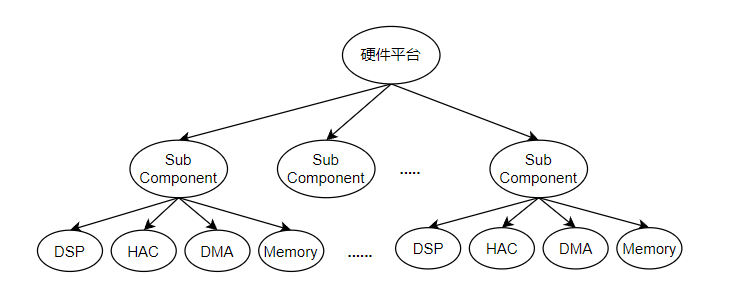
\includegraphics[width=1\textwidth]{硬件平台树状结构示意图.png}
    \caption{硬件平台树状结构示意图}
    \label{fig:badge}
\end{figure}

用户在进行仿真之前需要根据自己的需求去修改硬件平台配置文件,
硬件平台构建需要读取硬件平台配置文件并解析,系统所需的硬件平台配置文件包括
:V801.xml用来描述所有硬件模型之间的连接信息及Port信息、V801MemMap.xml
用来描述所有硬件模块模块与具体物理地址之间映射关系、V801MemPt.xml用来
描述内存模块的具体信息、V801Prop.xml用来描述所有需要实例化的模块包括
Processor和总线模块等等在实例化的时候的所需的所有具体信息、V801Route.xml
描述了所有实例化后的硬件模块之间的路由信息,将各个硬件模型通过总线连接形
成一个完整的硬件平台。在实际的用例仿真业务中,在进行用例仿真之前,仿真系统
先根据硬件平台配置文件对硬件平台进行构建,整个硬件平台的实例化的顺序如图5.1所示。

我们通过创建SaeSimulator单实例去实现整个平台初始化的功能,整个SaeSimulator
的类图如图5.2所示:

\begin{figure}
    \centering
    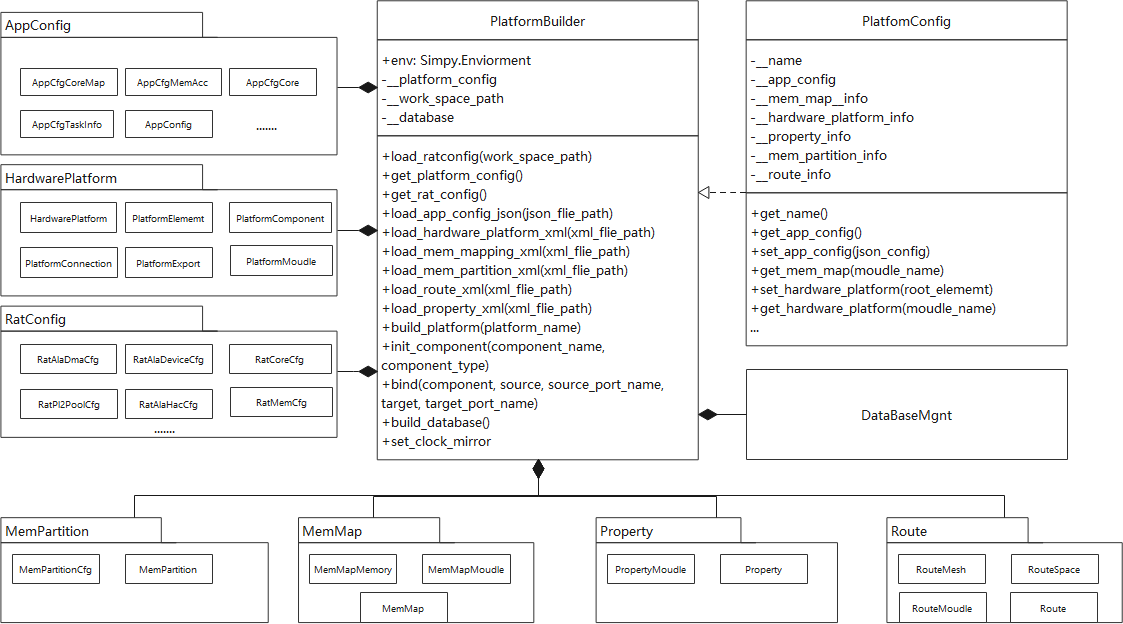
\includegraphics[width=1\textwidth]{硬件模块实例化模块类图.png}
    \caption{硬件模块实例化模块类图}
    \label{fig:badge}
\end{figure}

图5.2硬件平台实例化模块需要的类以及类之间关系构造的类图,在硬件平台实例化
模块中,我们在最外层通过SaeSimulator单实例调用load\_platform函数实现
PlatformBuilder类中对各个硬件配置文件的读取和解析以及实现硬件平台中
各个模型的实例化,PlatformBuilder类读取和解析硬件配置文件后,将硬件
配置信息存储到PlatformConfig类中各个属性中,并对每个属性设置get和
set函数,支持外部对类里面私有函数的设置和读取。最后,硬件模型的实
例化通过调用init\_component函数实现。

硬件模块实例化过程中,实现方式通过层次性的实例化。先按模块解析硬
件配置文件读取硬件配置信息。在逐层实例化各个模块。如硬件模块实例
化类图所示,每个包里是硬件的一部分,将包里的各个类根据读取的硬件
配置信息实例化,在实例化整个次外层的类,如AppConfig里的AppConfig
类。最后在init\_component函数中统一,最后通过bind函数将各个模块
通过路由信息中Port口连接起来。最后,通过DatabaseMgnt类实例化并
连接数据库文件。

% \subsection{TaskGraphManager模块设计与实现}

% TopLevel仿真平台的输入任务模型是实例级别的数据流图模型,任务之
% 间以数据为触发关系,任务之间的触发为实时触发。当任务的输入数据
% 全部就绪后,该任务实例才会开始执行,一旦任务执行完毕,其输出数
% 据被触发搬运。整体的任务的数据流图示例图如图5-2所示:
% \\
% \\
% \\
% \begin{figure}
%     \centering
%     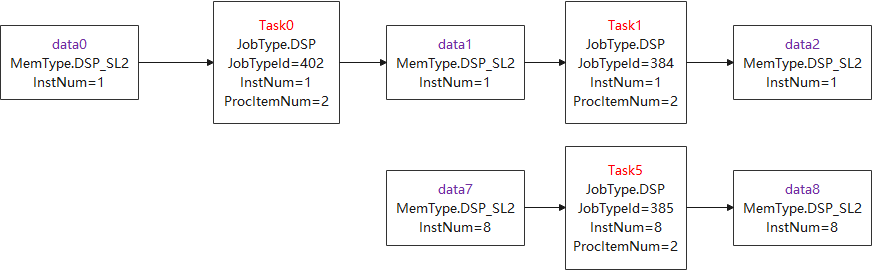
\includegraphics[width=1\textwidth]{任务数据流图示例图.png}
%     \caption{任务数据流图示例图}
%     \label{fig:badge}
% \end{figure}

% 仿真平台的任务用例输入类型是描述了所有任务相关信息的
% Excel文件,包括任务类型、任务执行的所属调度器、任务的
% 输入输出数据,数据的大小类型等等。平台初始化时通过
% SaeSimulaor单实例中的load\_task\_praph方法解析任务信息
% 文件,并通过TaskGraphMgnt类管理。TaskGraphManager类以及
% 相关类的类图如图5-3所示:

% \begin{figure}
%     \centering
%     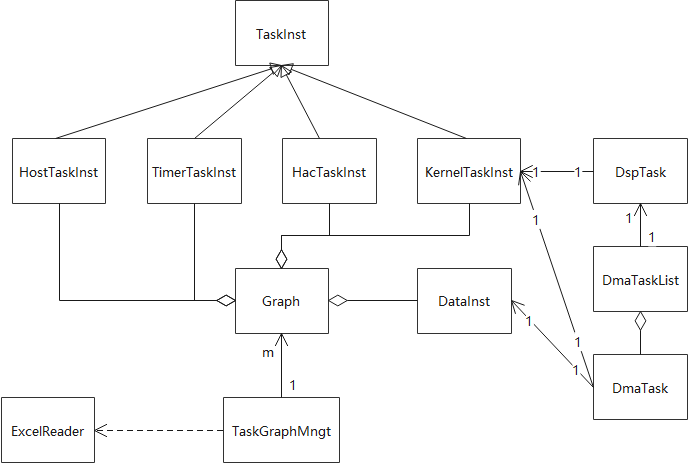
\includegraphics[width=1\textwidth]{TaskGraphMgnt模块类图.png}
%     \caption{TaskGraphMgnt模块类图}
%     \label{fig:badge}
% \end{figure}

% TaskGraphMgnt类通过ExcelReader类里的方法读取输入任务用
% 例的Excel表,将任务信息遍历读取,根据任务用例中任务具
% 体信息将任务根据自身信息生成不同类型的任务对象,将数
% 据信息生成DataInst类对象。在Graph类中由多种类型的节
% 点,如图5-2任务流图示例图所示每个节点之间双向连接。
% 为每个TaskInst节点配置input\_data和output\_data两个字
% 典,为每个DataInst节点配置producer和consumer两个字典,
% 在Graph类中读取任务实例和数据实例,并根据在任务用例文
% 件中任务和数据之间关系,分别将任务实例和数据实例填入
% 不同节点的各自的两个字典中,并且将数据和任务之间依赖
% 关系作为边设为edge\_list。在读取excel的过程中构造图
% 的结构,并不断地将TaskInst和DataInst以及结合他们之
% 间的映射关系加入Graph对象中。

% \section{仿真平台调度器模型设计与实现}

% 调度器模块通过Schdule模块读取TaskGraphMgnt对象里的Graph
% 任务图对象读取出来。Graph对象形式是有向无环图类型,Schdule
% 模块先遍历有向无环图,找到DAG图中没有入度的节点即为第一个
% 任务或数据,将实例输入到调度器模块,由TOP模块接收判断类型,
% 根据信息类型转发到SCH模块。

% TOP模块负责接收外部模块发送过来的任务图中实例信息以及硬件模
% 型处理任务完成后发送回来的响应,按照实例或者响应分开处理。
% RES模块负责管理各个核的私有内存(包括L1D、PL2);公共内存
% 资源(如SL2等);管理Device资源。SCH模块负责向RES模块申请
% 管理的硬件资源和内存资源。并将任务信息或数据信息发送到申
% 请好的硬件IP中进行处理。在SCH模块中对任务和数据处理流程
% 图如图5-4所示:

% \begin{figure}
%     \centering
%     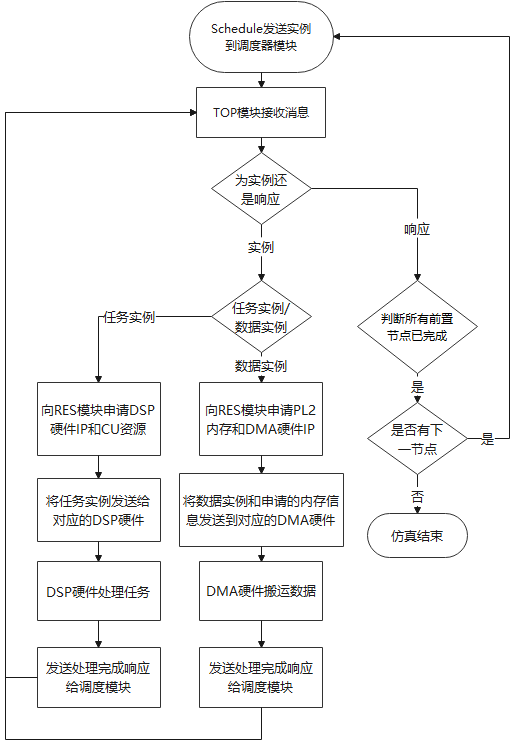
\includegraphics[width=0.55\textwidth]{调度器模块执行流程图.png}
%     \caption{调度器模块执行流程图}
%     \label{fig:badge}
% \end{figure}

% 调度器模块主要负责接收由Schedule模块中发送的实例级对象(包括数据
% 实例和任务实例)以及硬件模型执行完任务发送的响应消息。调度器模块
% 接收到如果是Schedule模块发送过来的实例级对象,调度器TOP模块接收
% 到实例对象后将实例对象发送到SCH模块进行资源的申请和任务的调度。
% 如图5-4所示实例对象分为数据实例和任务实例区分。当实例对象为数据
% 实例时,SCH模块根据数据实例中的数据信息将数据实例拆分成DMA任务
% 链,并为DMA任务链向申请DMA硬件资源以及每个DMA任务的所需的内存
% 空间(DMA任务为数据搬运任务)。当实例对象为任务实例时,任务实
% 例类型分为DSP任务和HAC任务,SCH模块根据任务信息申请空闲的硬件
% 资源和内存资源,将任务实例发送到对应的硬件模型中执行,任务的 
% 下一节点,则停止。当所有的任务都执行到没有出度的节点时,整
% 个仿真就结束了。这就是仿真平台的整个仿真流程经过调度模块调度
% 的整个流程。

\section{仿真平台Processor相关模块设计与实现}

仿真平台中Processor模块主要功能为:接收调度器模块发送过来的任务实例并
提取任务实例中中的任务信息,在具体的硬件实例上根据任务信息处理任务。
Processor模型类型主要分为DSP模块、DMA模块和HAC模块。下面详细阐述了仿真平台Processor
相关模块设计与实现。

\subsection{GeneralFifo模块设计与实现}

在整个仿真平台中,我们需要实现硬件模型能够在别的模块发送过来消息时
能够及时的对发送过来的消息进行处理,以及模型外部能够接收别的模型发
送过来消息的消息队列。这种消息队列主要用于Processor模块的流水线功能
的实现。这部分会在具体的Processor模型中阐述。
我们基于Simpy的仿真机制实现了GeneralFifo模块,并在整体仿真平台构建
时将此模块作为基础数据结构使用,与先入先出队列的整体逻辑类似。我们
在概要设计中简要介绍了GeneralFifo的整体执行流程。我们在这一节详细
介绍GeneralFifo的设计。GeneralFifo模块的类图如图5.3所示:
\begin{figure}
    \centering
    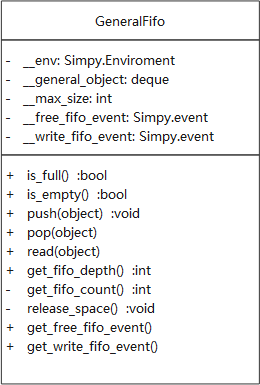
\includegraphics[width=0.45\textwidth]{GeneralFifo类图.png}
    \caption{GeneralFifo类图}
    \label{fig:badge}
\end{figure}

GeneralFifo模块的底层实现基于数据结构双向队列deque实现。整体实现
队列先入先出,并可以设置以及查询队列深度,查询队列中现有对象数量,
判断队列的状态。并基于Simpy的event机制实现了队列的Push和Pop功能。
每次将对象Push进队列时,将触发该队列的write\_fifo\_event,该event事
件触发时,会使在其他模块等待该事件触发的进程开始继续执行,从而实
现该队列一旦有对象存入,能够及时通知其他模块将对象从队列中取出进
行操作。同时,当队列为满时,其他模块只需等待free\_fifo\_event事件
触发,其他模块即可继续向Fifo中Push对象。这样就是实现不同模块之
间基于GeneralFifo的信息传输的功能,以及实现一个模块等待信息的
场景。在仿真平台中所有模块之间交互以及Processor模块的实现都是
基于GeneralFifo实现的。

\subsection{Processor模块设计与实现}
Processor模块主要实现对三种基础硬件模型(DSP、HAC和DMA)的建模
以及Processor模块与调度器模块之间的交互。在实现三种基础模型的
建模之前,我们实现ProcessorBase类,通过ProcessorBase类所有
Processor模型的基础功能进行实现。

平台中所有模型都是以GeneralModule类为基类实现,GeneralModule
模块是统一所有已实例化的模型并将这些模型联系起来的模块。GeneralModule
模块实现了平台信息和实际硬件模型信息的联系,并为每个模型模块创
建了Log文件,在各模块中可以调用其基类GeneralModule类中的log方
法去记录log信息,并统一设置整个仿真过程中的log等级,以应对不同情
况下的业务仿真;GeneralModule模块中也将数据库模块和具体模块之间
联系起来,在各模块中可以调用其基类GeneralModule类中的message
方法去记录信息并存储到数据库中。GeneralModule模块关系类图如下图所示:

\begin{figure}
    \centering
    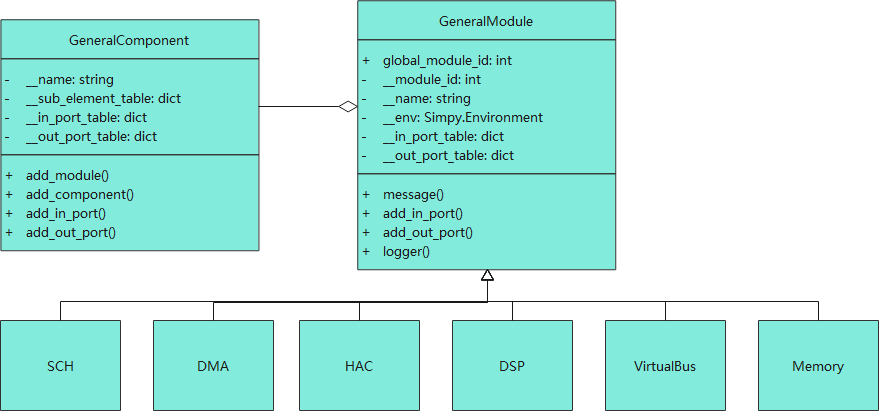
\includegraphics[width=0.7\textwidth]{GeneralModule关系类图.png}
    \caption{GeneralModule关系类图}
    \label{fig:badge}
\end{figure}

Processor模块具体实现三种模型的功能建模,分别为DMA模型、DSP模型
以及HAC模型。DMA模型的主要功能是要实现数据搬运功能,为DSP模型中
的具体执行将数据从SL2搬运到具体DSP组的PL2中或者数据处理结束后从
PL2搬运到SL2,再或者仅仅只进行内存中的数据交换。DSP模型模拟核的
执行过程的流程,主要执行数据的处理。硬件加速器(HAC:HardWare 
Accelerator)模型模拟了从数据搬运到数据处理再到数据搬出的整体
流程。HAC主要为了执行某一种特定的执行多次的硬件任务,任务在HAC
上执行速度较快,任务的整个执行流程均在HAC硬件上完成。

调度器模块需要将任务分发到调度器向RES模块申请的具体的硬件模型。
但由于整个平台软硬件设计分离,调度器模块无法获取硬件平台整体构
建信息,无法直接与硬件模块相互交互。因此我们需要一个模块实现调
度器模块与具体硬件模型之间的交互,为此我们在Processor模块中设
计了单实例ProcessorMgnt,用于实现交互功能。Processor模块以及
相关模块关系如图5.5所示:

\begin{figure}[!h]
    \centering
    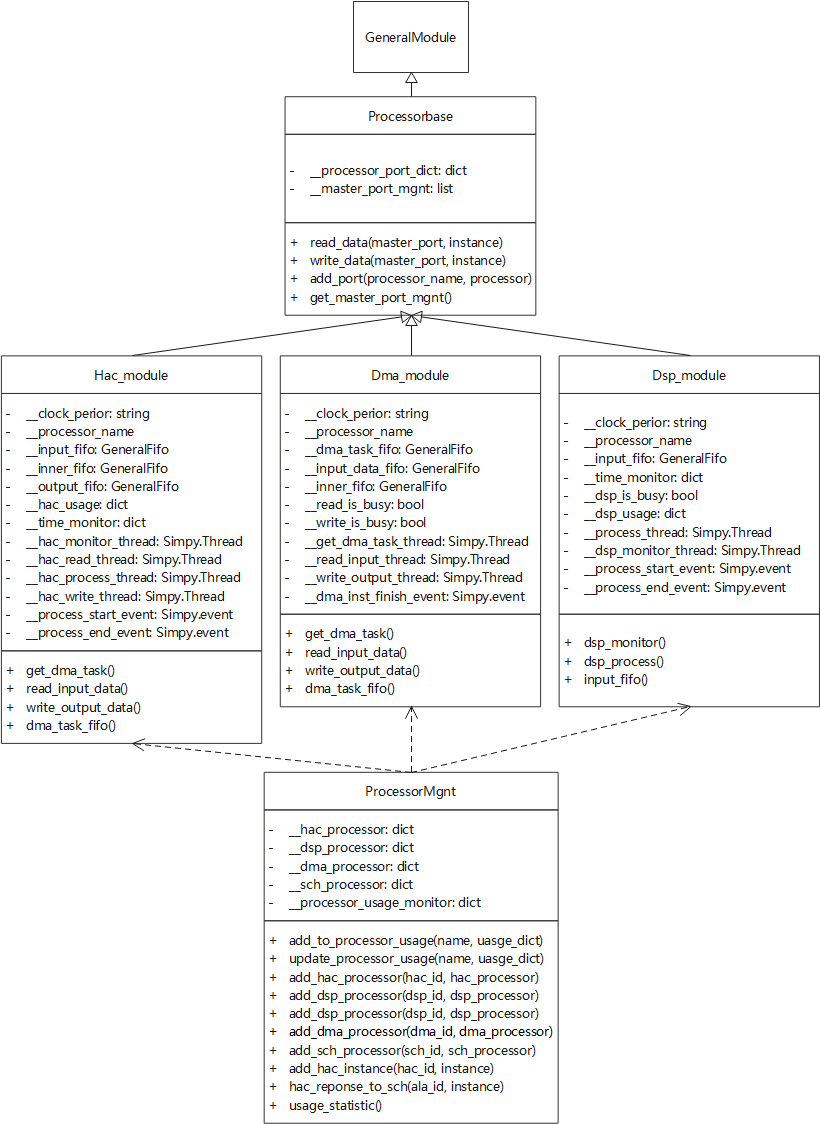
\includegraphics[width=0.8\textwidth]{Processor模块类图.png}
    \caption{Processor模块类图}
    \label{fig:badge}
\end{figure}

图5-7显示了ProcessorMgnt、三种具体的Processor模型、所有
Processor模型的基类ProcessorBase以及几者之间的关系。在
ProcessorMgnt模块中,各个模块在实例化的时候通过调用单实例的
对应方法通过相应类型的dict去记录,dict以模型名为键值。当其
他模块模块之间需要进行交互时,就可以通过调用ProcessorMgnt
单实例相应方法去访问对应字典,通过模型名就可以取到相应的模
型对象,从而进行交互。

三种基础的硬件模型以ProcessorBase为基类。ProcessorBase类实
现了几种基础硬件模型的公有方法:如实例化Port、读数据、写数
据、管理MasterPortMgnt等等。在介绍具体的Processor模型实现之前,
我们先介绍在仿真平台中传输的数据类型。

在仿真平台中传输的数据主要包括RwObject、Burst以及Flit三种。在
最外层硬件模块中传输的数据的数据类型为RwObject,数据在总线上
传输的数据格式为Flit。图5.6为三种数据类型的类图,以及图5.7
为三种数据类型之间的关系图。

\begin{figure}
    \centering
    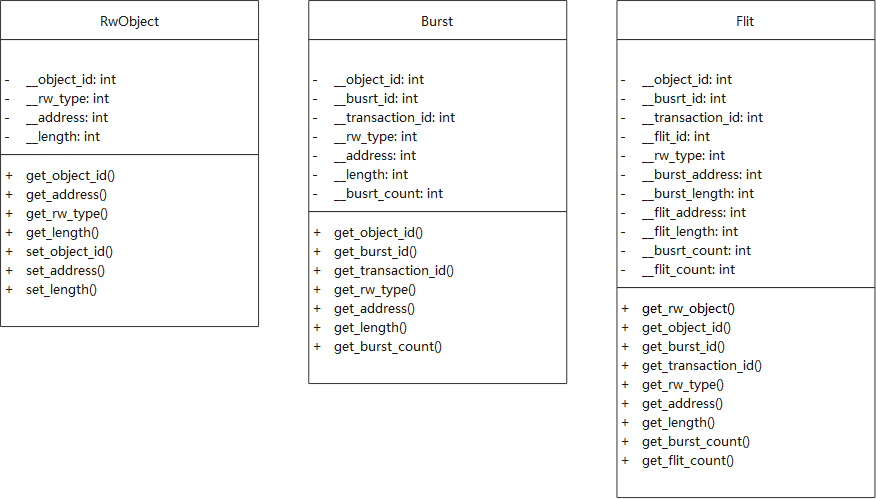
\includegraphics[width=1\textwidth]{三种数据类型类图.png}
    \caption{三种数据类型类图}
    \label{fig:badge}
\end{figure}

\begin{figure}
    \centering
    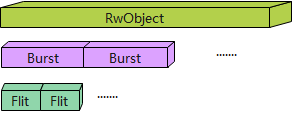
\includegraphics[width=0.6\textwidth]{数据类型关系图.png}
    \caption{数据类型关系图}
    \label{fig:badge}
\end{figure}

接下来介绍三种基础硬件模型的具体实现:首先我们介绍DSP模块
的功能实现。DSP模拟的是核的处理过程,在
仿真过程系统只需模拟真实的处理时延即可。调度器模块将任务用
例通过ProcessorMgnt模块发送到DSP模块的input\_fifo中,在模
型中process\_thread一直在等待输入,FIFO中一旦有对象传入,
进程就开始进行处理。处理时延在输入的任务用例表中已有,我
们只需从任务用例中取出时延信息,在乘以硬件的时钟频率即可
得到需要停止的仿真时间。

接下来我们介绍DMA模块的功能实现。DMA模块需要完成的对DSP
模块需要处理数据的搬入搬出,将数据从SL2内存中搬入DSP模
块的PL2内存中的过程称为前搬移,将数据从PL2内存搬运到SL2
的过程称为后搬移。数据的搬入搬出,DMA模块通过任务用例中
的地址和数据大小信息创建RWObject,通过MasterPortMgnt经
过总线进行传输,在总线上的传输在后续介绍总线互联模块的
时候详细阐述。我们创建两个线程分别用来处理数据的搬入和
数据的搬出,以及创建一个线程获取DMA任务实例和控制总体
的流水线深度。DMA模块通过各级线程以及线程之间的FIFO实
现流水线。每一级线程均从FIFO中取任务实例,执行完任务
实例,再将任务实例发到下一级的FIFO中,从而实现流水线
。DMA模块的流水线执行时序图如图5.8所示:

\begin{figure}
    \centering
    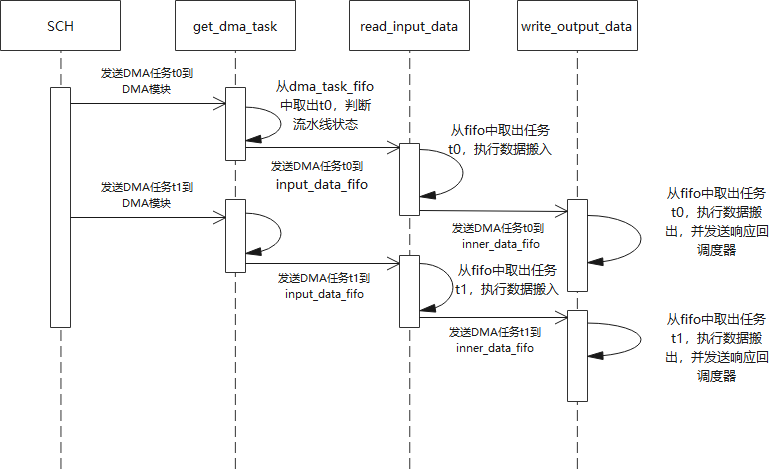
\includegraphics[width=1\textwidth]{DMA模块流水线时序图.png}
    \caption{DMA模块流水线时序图}
    \label{fig:badge}
\end{figure}

DSP模块负责完成输入数据的处理。我们在仿真平台中只完
成处理时延的仿真,并不真实的进行数据的处理。前搬移
任务、DSP任务以及后搬移任务形成一整个任务流程,当
前搬移DMA任务完成时直接触发相应的DSP任务,发回调
度器的响应只用来释放DMA任务申请的系统资源。

HAC模块是用来处理专用任务的硬件。一种HAC只用来执
行一种任务,用来加速任务的处理。HAC硬件模块中需
要完成数据的搬入、处理以及搬出的一整套流程。HAC
模块接收调度器模块发送过来的HAC任务实例,HAC任
务实例中记录着输入数据、处理时延以及输出数据等
相关信息。HAC模块通过三级流水实现数据搬入、数
据处理以及数据搬出的功能。HAC模块的三级流水时
序图如图5.9所示:

\begin{figure}
    \centering
    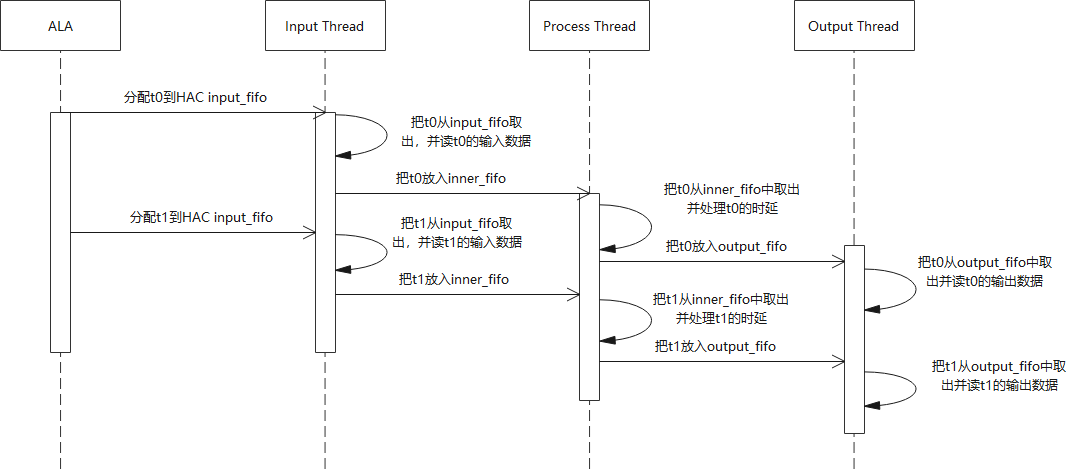
\includegraphics[width=1\textwidth]{HAC模块三级流水时序图.png}
    \caption{HAC模块三级流水时序图}
    \label{fig:badge}
\end{figure}

此外,Processor模块还在DSP模型和HAC模型中实现统计核工作
的时间片的通过。通过dsp\_monitor\_thread和hac\_monitor\_thread
两个进程分别去统计DSP模型和HAC模型的执行时间片。以DSP模块
为例,DSP模块在从FIFO中取出任务实例时触发process\_start\_event,
处理完时延后触发process\_end\_event。这两个事件都会使挂起的进程
开始执行,从而统计DSP模型每次执行的时间片区间。HAC模型内部工
作时间块统计与之相同。

% \subsection{Port模块设计与实现}
% 在仿真平台中,在不同模块之间通过总线进行通讯,而总线在不同模块上
% 的端口则是Port模块。针对端口设计的可扩展性,我们以Moudule Port 
% Base为基础,采用Master/Slave方式。在仿真平台中,所有端口采用双
% 向绑定机制,即在Master端可以调用Slave端的方法.

% 仿真平台中现在主要有两种模块间通讯接口,一种为硬件模型模块间的接
% 口:Virtual Master Port和Virtual Slave Port,另一种是总线内部子
% 模块之间的流水线通讯接口VBusPipeLineMasterPort与VBusPipeLineSlavePort。
% Port模块的关系类图如图5-13所示:

% \begin{figure}
%     \centering
%     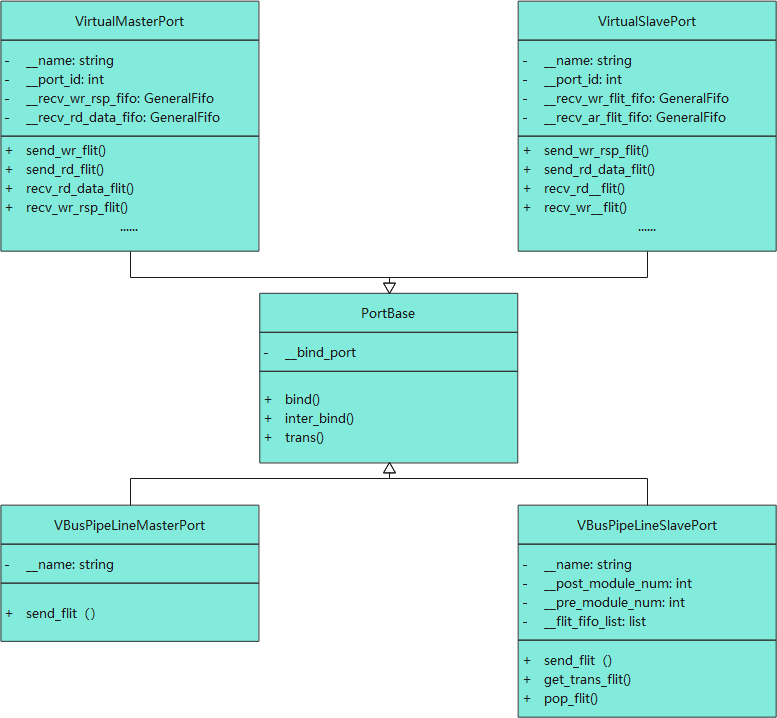
\includegraphics[width=1\textwidth]{Port模块关系类图.png}
%     \caption{Port模块关系类图}
%     \label{fig:badge}
% \end{figure}

% Master Device在硬件实例化的时候创建对应的VirtualMasterPort,
% Slave Device在硬件实例化的时候创建对应的VirtualSlavePort。
% Master Device一般是硬件Processor模型,在5.3.2节所介绍,
% 硬件IP实例化时通过调用ProcessorBase的方法add\_port创建
% Port端口。Slave Device一般值得是Memory模块。在平台构建
% 时,VirtualMasterPort和VirtualSlavePort通过硬件平台配
% 置表上的信息进行绑定。这两种端口都由PortMgnt进行管理,
% 如上一小节所说,Master端通过MasterPortMgnt调用
% send\_wr\_flit和send\_rd\_flit方法向sendWrFlitFifo和
% sendARFlitFifo发送写地址请求、写数据请求和读地址请求,
% Slave设备调用send\_wr\_rsp\_flit和send\_rd\_data\_flit和send
% 方法向recvWrRspFifo和recvRdDataFifo返回读数据和写响应。
% VbusPipeLineMasterPort和VbusPipeLineSlavePort模块在BUS
% 模块设计中介绍。

% \subsection{BUS模块设计与实现}

% 在仿真平台硬件模块中,所有数据信息的传输都是通过总线模块进行,
% 所有的数据传输都是通过Port模块拆分封装成Flit格式的数据包经过
% 总线模块从一个硬件模块发送到另一个硬件模块。
% Virtual Bus模块由多个模块构成,每个模块负责不同的功能。BUS模块
% 整体架构图如4.2.3节图4-5所示。模块主要分为三种:总线输入模块
% InputStage、总线处理模块(包括各个通道的译码器和仲裁器等)以
% 及总线输出模块TLOutputStage。每一个Master Device或Slave Device
% 都通过总线端口连接到Virtual Bus中对应的InputStage模块或
% TLOutPutStage模块。

% 在传输过程中,Master设备发起的读写请求通过Port端口传入到
% InPutStage模块当中,InputStage通过Fifo将请求发送到对应的译码
% 器,译码器经过地址译码将请求发送发送到对应的仲裁器,仲裁器根
% 据优先级将写入数据发送到对应的TLOutPutStage进而传输到Slave 
% Device或者取数据发送回InputStage进而返回Master Device。

% 总线处理模块的主要功能是地址译码、优先级仲裁以及模拟每个
% flit的传输。BUS模块中一共有四种通道,分为写通道、读地址通道、
% 写响应通道和读数据通道。每个通道都有一套独立的译码模块和仲裁
% 模块,各个模块之间通过端口连接,使用Fifo实现数据消息的传输。
% 每个Master端口对应一个WDecoder、一个RDecoder、一个ARDecoder
% 以及一个BDecoder,一个Slave端口对应一个WArbiter、一个RArbiter、
% 一个ARArbiter以及一个BArbiter。通过一个管理模块将一种功能的所有
% 模块聚合到一起进行管理。

% BUS模块的的类图如图5-14所示:
% \\
% \\
% \\
% \\
% \\
% \\

% \begin{figure}
%     \centering
%     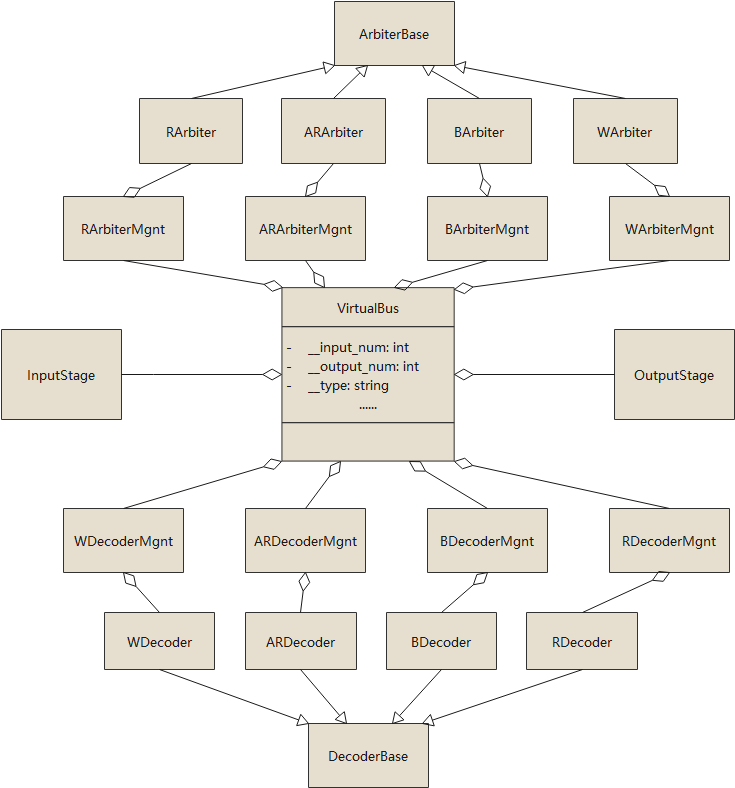
\includegraphics[width=1\textwidth]{BUS模块关系类图.png}
%     \caption{BUS模块关系类图}
%     \label{fig:badge}
% \end{figure}

% InputStage模块在整个BUS模块中的作用是作为外部Master Device与
% 内部沟通的桥梁。主要的工作流程是接收Master Device发送来的flit,
% 并将flit发送到对应的译码模块;以及将来自仲裁模块的flit发送回
% Master Device。主要通过四个不同的FIFO接收不同种类的flit
% (写请求、读请求、写响应、读响应)。

% OutputStage模块在整个BUS模块中是模块内部与Slave设备沟通的桥梁。
% 主要的工作的流程是接收来自总线模块内部发送来的flit,并将flit发
% 送到对应的Slave设备的Port模块;或者将Slave设备Port返回的响应发
% 送到对应的Decoder模块上。同样也是通过四个不同的FIFO接收四种类
% 型的flit。

% BUS模块的每个通道都有独立的译码模块,但读数据通道和写响应通道的
% 译码模块都是对响应的译码,处理逻辑相同,我们将读数据通道和写响
% 应通道的译码器模块合二为一。在平台中,一个总线模块对应一个Port
% 模块。同一个通道的Decoder由一个DecoderMgnt进行管理。BUS模块在
% 实例化的时候会读取平台解析的memory mapping信息并将这些信息汇
% 总成一个路由表。当flit到达译码模块时,译码模块通过路由表寻址
% 到flit目的地址所对应的Slave Device的Arbiter模块,并将flit发
% 送到对应的Slave Device的Arbiter模块。在译码过程中一个Burst
% 的所有的flit只有第一个到达译码模块的flit需要进行译码过程,
% 接下来译码模块会记录该Burst对应的Arbiter模块,当其余flit发
% 送过来时就不需要重复译码。

% Arbiter模块的作用是对同一通道来自不同Decoder模块发送过来的
% flit进行传输顺序的仲裁。现在仲裁模块的算法采用的轮询算法,
% 但在轮询算法的基础上回尽可能的保证同一个Burst的flit能够连
% 续发送。一个通道的所有Arbiter都会通过各自的ArbiterMgnt进
% 行管理。

\section{仿真平台Memory模块设计与实现}

仿真平台的Memory模块主要实现接收Master设备通过总线互联模块发送
过来的读写请求flit,根据Bank位宽拆成对应的Bank操作发送到对应地
址的Bank的FIFO上。

Memory模块提供交织的Bank。这些Bank模块根据地址相互交织,每个Bank
的偏移地址与Bank位宽相同。仿真平台中Memory模块Bank模块设计为4个Bank,
Bank位宽为256字节的设计方案。Memory模块在实例化的时候创建4个Bank模块,
Memory模块可以同时处理不同的Bank模块上的Bank操作,但每个Bank模块同时只
能处理一个Bank操作。Bank模块的交织方案如图5.10所示:
\\
\\

\begin{figure}
    \centering
    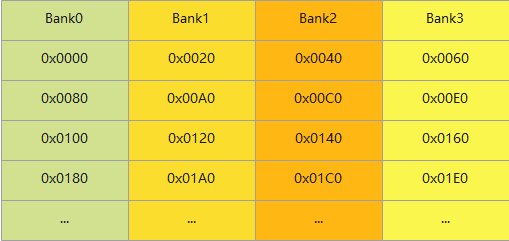
\includegraphics[width=0.8\textwidth]{Bank模块交织方案.png}
    \caption{Bank模块交织方案}
    \label{fig:badge}
\end{figure}

Bank模块在初始化时创建读写Bank线程。读写Bank操作完成向对应的SlavePort
发送读写响应flit。Memory模块接收SlavePort发送过来的flit,因为对读写请
求的操作不同,Memory模块会根据读写请求的区别分到不同的FIFO中。Memory对
发送过的flit的处理流程图如图5.11所示:

\begin{figure}
    \centering
    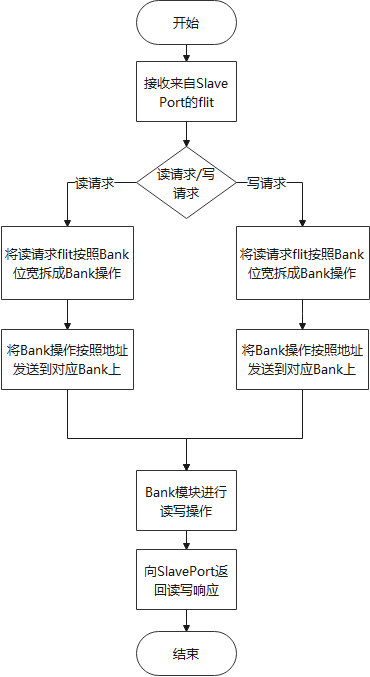
\includegraphics[width=0.49\textwidth]{Memory模块处理流程图.png}
    \caption{Memory模块处理流程图}
    \label{fig:badge}
\end{figure}

Bank写操作结束时,Memory模块会统计一个Burst完成flit的数量,当最后一个flit
操作完成后会统一发送一个写响应回SlavePort。而Bank读操作则时完成一个flit就
发送一个flit的读响应到SlavePort上。最后由总线互联模块发送回发送读写请求的
Master设备,完成一整个读写操作。

\section{设计空间探索相关模块的设计与实现}

设计空间探索模块实现的功能是对我们所需要探索的设计目标在设计空间中寻找最优
或者是较优设计。设计空间模块主要分为三个模块:训练集生成模块、预测模型生成
模块以及遗传算法探索模块。设计空间探索模块的整体流程图如图5.12所示:

\begin{figure}
    \centering
    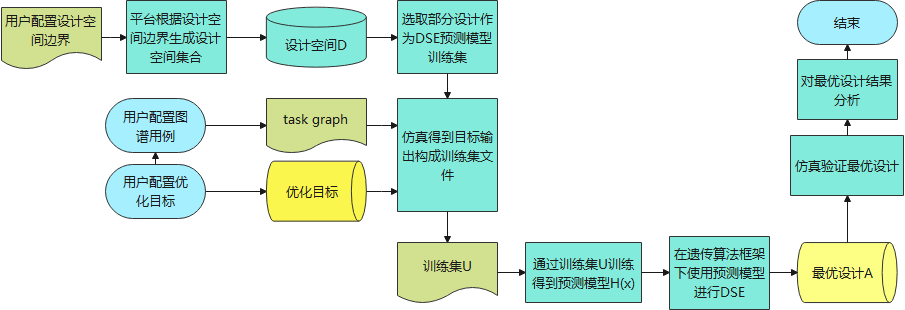
\includegraphics[width=1\textwidth]{设计空间探索模块整体流程图.png}
    \caption{设计空间探索模块整体流程图}
    \label{fig:badge}
\end{figure}

接下来主要介绍训练集生成模块和预测模型生成模块的具体设计与实现以及设计空间探索结果分析。

\subsection{训练集生成模块的设计与实现}

训练集生成模块主要包括设计参数、设计边界与目标值的选取、设计空间的生成以及根据设计空间
以及目标值生成下一步预测模型所需要的训练集文件。在仿真平台中我们选取可配置参数作为我们
的设计参数,并根据实际情况设置各个设计参数的设计边界,具体设计参数及设计边界如表5.1所示:

\begin{table}[!h]
    \centering\normalsize
    \caption{仿真平台设计空间}
    \begin{tabular}{c|c|c}
    \hline
    \textbf{设计参数} & \textbf{设计参数取值}         & \textbf{数量} \\ \hline
    PL2 Pool Size & 100000-190000: 10000+   & 19          \\ \hline
    PL2 Unit Size & 10-50: 10+              & 5           \\ \hline
    SL2 Pool Size & 1500000-1850000: 50000+ & 7           \\ \hline
    SL2 Pool Size & 10-50: 10+              & 5           \\ \hline
    Cu Num        & 1-5: 1+                 & 5           \\ \hline
    Dsp Num       & 4-16: 2+                & 7           \\ \hline
    BUS Bit Width & 64-512: 64+             & 8           \\ \hline
    \end{tabular}
    \end{table}

我们选取了七个参数作为我们设计空间探索的设计参数值,设计参数分别为:PL2内存池大小、PL2每个内存单元大小、SL2内存池大小、SL2每个内存单元大小、Cu数量、Dsp数量以及总线位宽。这些参数均会影响最后仿真结果。这些设计参数的组合最后构成的设计空间包括了超过56万个不同的设计配置。

我们设计空间探索主要探索的方向主要是时延以及核的使用方面。我们最终选取了仿真时延、每个TTI核的利用率、每个TTI核的一致性为我们设计空间探索的目标值。接下来我们说明每个目标值的统计标准。仿真时延在数据库文件中有着直接的记录,我们只需直接提取数据库中的信息即可,核的利用率在数据库中记录了每个时间片(0.002TTI)的核的利用率,记录方法已在5.1.5节介绍。我们只需将数据库中信息整合每个TTI的核的利用率即可。核的一致性指的是在同个TTI内所有核的利用率的方差,我们需要将之前统计的核的利用率进行计算即可。这就是我们设计空间探索的优化目标值。

我们生成训练集的流程图如图4.9所示。我们将RatConfig表中需要改变的参数值单独设置一页Config
表,并将这一页的值与整张表中的相关的值相关联,通过openpyxl插件去修改Config表中的参数。
这样我们就可以通过脚本自动改变设计参数去运行仿真,仿真结束后提取数据库中目标值信息,处理
后将设计参数和目标值一同输出到训练集文件中。我们训练集文件大小为6000,生成训练集模块一共
运行了6000次仿真。训练集文件格式如图5.13所示:

\begin{figure}
    \centering
    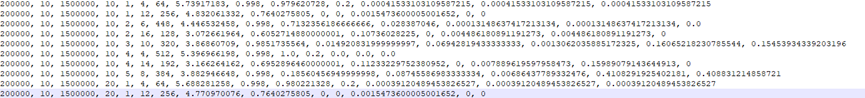
\includegraphics[width=1\textwidth]{训练集文件格式示例.png}
    \caption{训练集文件格式示例}
    \label{fig:badge}
\end{figure}

\subsection{预测模型生成模块设计与实现}

我们在遗传算法进行设计空间探索过程中,在不断迭代每一代种群时如果每一次都要进行仿真从而得到对应设计参数的目标值,整体设计空间探索的时间就会十分的漫长。于是,我们使用机器学习生成的预测模型去代替实际的仿真平台去进行遗传算法设计空间探索的过程,这样能够大大减少设计空间探索的时间。

我们多目标预测模型采用先对不同目标值分别进行机器学习的过程,得到对应7个目标值的7个预测模型。我们将这7个预测模型通过一个multi\_model类集成到一起,通过multi\_model类的方法我们可以通过输入设计参数从而得到相应的目标值。多目标预测模型集成的各个目标值的准确度(以R2确定系数为标准)如表5-2所示:

\begin{table}[!h]
    \centering\normalsize
    \caption{多目标预测模型误差值}
    \begin{tabular}{|c|c|c|c|}
    \hline
    \textbf{时延}       & \textbf{TTI0核利用率} & \textbf{TTI1核利用率} & \textbf{TTI2核利用率} \\ \hline
    0.99824568        & 0.9999998         & 0.9982341         & 0.9873023         \\ \hline
    \textbf{TTI0核一致性} & \textbf{TTI1核一致性} & \textbf{TTI2核一致性} & \textbf{}         \\ \hline
    0.8638929         & 0.9831229         & 0.8559540         &                   \\ \hline
    \end{tabular}
    \end{table}

从表中我们可以清楚的看出对于多个目标值而言,每个目标值的误差值不超过0.15。整个预测模型可以
比较高效精准的预测出目标值,与真实仿真平台的仿真结果相差不大,为了更加精准的看出预测模型
与仿真平台的结果差距,我们将1200次仿真结果作为验证集与预测模型进行对比,仿真结果与预测结果
对比如图5.14所示:

\begin{figure}[!h]
    \centering
    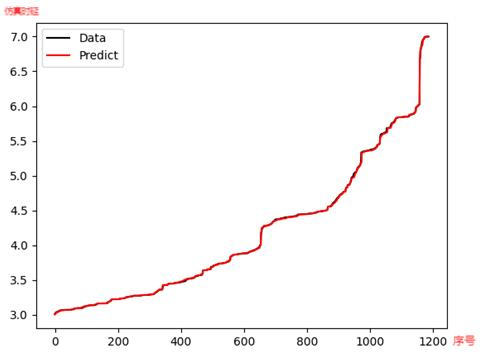
\includegraphics[width=0.45\textwidth]{仿真结果与预测结果对比图1.png}
\end{figure}

\begin{figure}[!h]
    \centering
    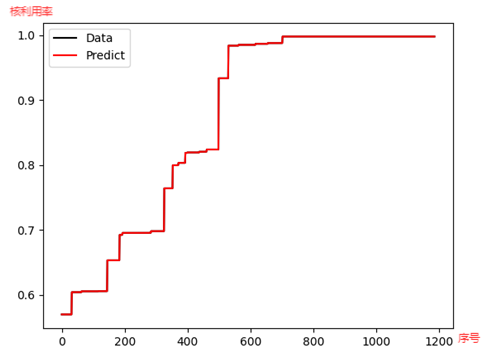
\includegraphics[width=0.45\textwidth]{仿真结果与预测结果对比图2.png}
\end{figure}

\begin{figure}[!h]
    \centering
    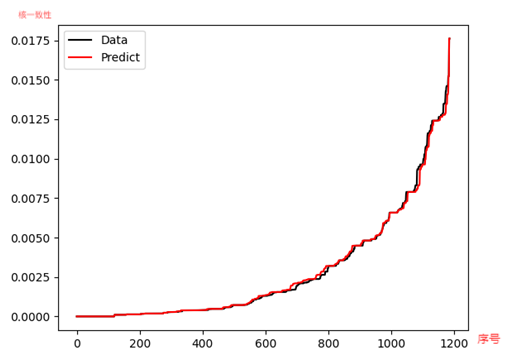
\includegraphics[width=0.45\textwidth]{仿真结果与预测结果对比图3.png}
    \caption{仿真结果与预测结果对比图}
\end{figure}

\subsection{设计空间探索结果分析}

在得到多目标预测模型之后,我们将使用多目标预测模型使用遗传算法进行设计空间探索。遗传算法执行过程中我们
使用NGSA-Ⅱ,我们通过交叉变异等操作产生子代,将父代和子代放到一起进行快速非支配排序,构造出不同等级
的非支配解集。按照需求计算每一代所有个体的拥挤距离,并根据拥挤度比较构造下一代种群。

遗传算法我们遗传代数设置为200代,每代种群数量为50,变异概率为0.1。最终演化种群中的每个基因型经过仿真平
台仿真运行得出相应的目标值。最终我们得到了50个设计方案,并且将这50个设计方案在仿真平台上进行仿真,得到
了相应的目标值。我们根据这50个设计方案以及对应的目标值进行探索,得到了以下结论。

我们先将三个方面的50个目标值与原始设计相对比得到图5.15。

\begin{figure}
    \centering
    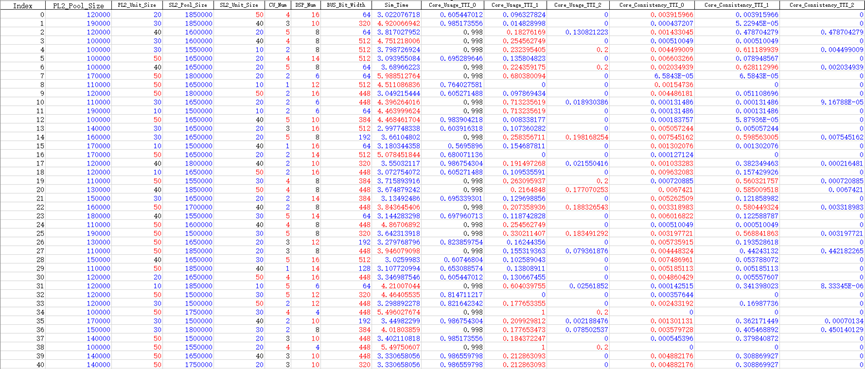
\includegraphics[width=0.8\textwidth]{设计空间探索结果仿真目标值结果对比图.png}
    \caption{设计空间探索结果仿真目标值结果对比图}
    \label{fig:badge}
\end{figure}

根据图5.15我们可以找到对于这几个方面单独而言最优的几个设计方案,我们基于优化目标将所有方案的结果
以及原始设计方案放到一起进行比较。比较结果如图5.16至5.18所示:

\begin{figure}
    \centering
    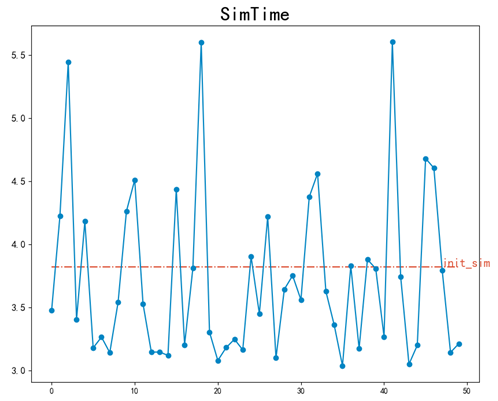
\includegraphics[width=0.5\textwidth]{50组设计方案时延结果对比.png}
    \caption{50组设计方案时延结果对比}
    \label{fig:badge}
\end{figure}

图5.16中横坐标为设计方案序号,纵坐标为仿真时延,红色虚线为初始设计方案及其对应的仿真时延。
由图5.16及对应序号的设计方案可以看出序号为35、43、20、27、14、7、48、12、13、23的方案较好。并且通过各个设计方案值之间的结果对比可以得出影响时延结果的主要因素为核的数量以及总线位宽等等。

\begin{figure}
    \centering
    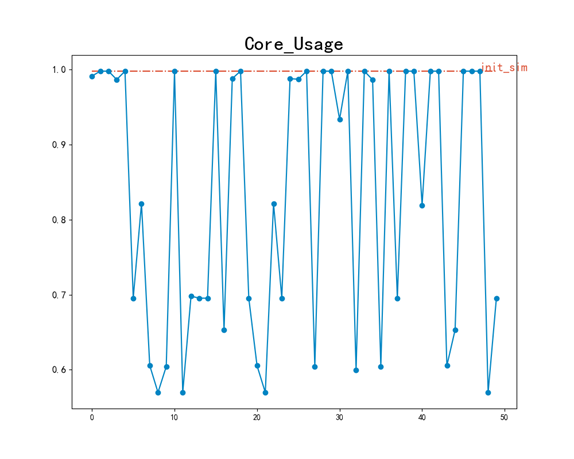
\includegraphics[width=0.6\textwidth]{50组设计方案核利用率结果对比.png}
    \caption{50组设计方案核利用率结果对比}
    \label{fig:badge}
\end{figure}

由图5.17及对应序号的设计方案可以看出序号33、28、42、29、47、39、36、38、4、26的方案较好。
并且通过各个设计方案之间的结果对比可以得出影响核利用率的主要因素为核的数量及CU数量等等。

\begin{figure}
    \centering
    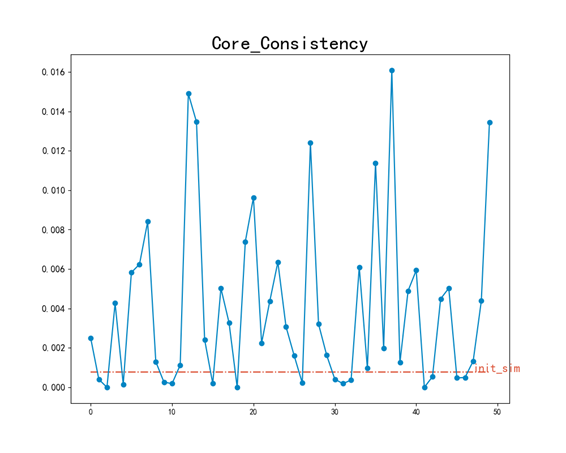
\includegraphics[width=0.6\textwidth]{50组设计方案核一致性结果对比.png}
    \caption{50组设计方案核一致性结果对比}
    \label{fig:badge}
\end{figure}

由图5.18及对应序号的设计方案可以看出序号2、18、41、4、31、15、10、26、9、32的方案较好。
并且通过各个设计方案之间的结果对比可以得出影响核利用率的主要因素为核的数量及CU数量等等。
而且对比图5.16和图5.17可以发现核利用率和核一致性的优化方向和影响因素大致相同。

但针对多个目标值同时考虑而言,我们需要找到多个目标值均衡的几个设计方案。从图5.16至图5.18可以看出
时延和核的利用率优化方向相反。仿真时延低的几种方案,设计参数中Dsp数量较大,但由于Dsp数量较大,
导致核的利用率和一致性效果较差。而核的利用率和核的一致性优化方向相同,最优的几个设计方案设计参数
大致相同。于是我们就核利用率和仿真时延两个方面进行考虑,结果图如图5.19所示:

\begin{figure}
    \centering
    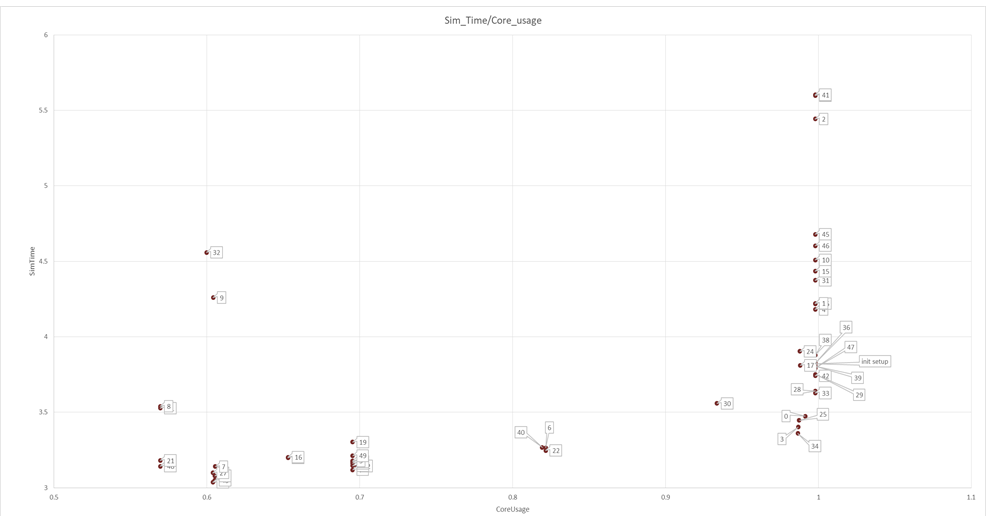
\includegraphics[width=1\textwidth]{仿真平台结果分析图.png}
    \caption{仿真平台结果分析图}
    \label{fig:badge}
\end{figure}

从图5.19中我们可以找到6种方案在仿真时延和核利用率两个方面表现都很优秀的设计方案如表5.3所示:

\begin{table}[]
    \centering\footnotesize
    \caption{最优设计方案设计参数}
    \begin{tabular}{|c|c|c|c|c|c|c|c|}
    \hline
    Index & PL2\_Pool\_Size & PL2\_Unit\_Size & SL2\_Pool\_Size & SL2\_Unit\_Size & Cu\_Num & Dsp\_Num & BUS\_Bit\_Width \\ \hline
    33    & 140000          & 30              & 1550000         & 20              & 4       & 8        & 448             \\ \hline
    25    & 170000          & 40              & 1650000         & 10              & 5       & 10       & 320             \\ \hline
    3     & 170000          & 20              & 1800000         & 50              & 2       & 10       & 512             \\ \hline
    42    & 100000          & 20              & 1800000         & 20              & 4       & 8        & 512             \\ \hline
    0     & 100000          & 10              & 1750000         & 50              & 4       & 10       & 128             \\ \hline
    25    & 170000          & 30              & 1650000         & 10              & 5       & 10       & 320             \\ \hline
    \end{tabular}
    \end{table}

从整体设计参数以及目标值的变化,我们可以看出增加Cu数量可以增快仿真速度,提高总线带宽可以使核的利用率提高同时还可以增快仿真速度。

\section{本章小结}

本章的工作主要是在第四章概要设计的基础上,详细的阐述了仿真平台中硬件平台
的构建、Processor模块以及Memory模块的具体实现,介绍了设计空间探索流程的
具体设计和实现。包括硬件平台的搭建、Processor
模块和Memory模块设计和实现,最后基于设计实现的仿真平台,阐述了设计空间流程
的设计和实现。实现整个仿真平台的搭建以及基于仿真平台的设计空间探索流程,
最后得到了设计空间探索结果种群,并对最终得到的设计空间探索结果进行了分析,得到了最终的
最优设计方案以及设计方案优化的目标

在本章基础上,下一章节我们将完成对仿真平台的测试。